\newpage
\chapter{Particle detection and event selection}
\mbox{}\vspace{-\baselineskip}
\label{chap:event_selection}

\section{Experiment overview}

The Spin Physics Detector (SPD) collaboration proposes to install a universal detector in the second interaction point of the NICA collider to study the spin structure of the proton and deuteron and other phenomena using a unique opportunity to operate with polarized proton and deuteron beams at collision energies up to $\sqrt{s_{pp}}=$27~GeV and $\sqrt{s_{NN}}=$13.5~GeV and luminosity values up to $10^{32}$~cm$^{-2}$~s$^{-1}$ and $10^{31}$~cm$^{-2}$~s$^{-1}$, respectively\cite{TDR_SPD,SPDproto:2021hnm,SPD_1st_stage,Arbuzov:2020cqg}.

 %27~GeV and luminosity values up to $\mathcal{L}=10^{32}$~cm$^{-2}$~s$^{-1}$\cite{TDR_SPD,SPDproto:2021hnm,SPD_1st_stage,Arbuzov:2020cqg}.

The SPD experimental setup is designed as a universal 4$\pi$ detector with advanced tracking and particle identification capabilities. General layout of the SPD detector in presented in Fig.~\ref{fig:spd_layout}. The complete detector setup will include the following components. 
\begin{itemize}

\item The Silicon Vertex Detector (SVD) is responsible for the precise determination of the primary particle interaction point and measurements of the secondary vertices from the decays of short-lived particles.

\item The Straw tube-based Tracking system (ST) with the purpose to reconstruct tracks of primary and secondary charged particles, to measure their momenta with high precision, based on track curvature in magnetic field, and to contribute to particle identification via energy deposition measurements.


\item The Time-of-Flight system (TOF) intended to distinguish between charged particles of different masses ($\pi$/K/p) in the momentum range up to a few GeV/c. Possible use of the Focusing Aerogel Ring-Imaging Cherenkov detector (FARICH) will extend this range significantly in the end-caps. 

\item A sampling Electromagnetic Calorimeter (ECal) to detect photons and electrons.  

\item The Range (muon) System (RS) is planned for muon identification and can also act as a rough hadron calorimeter. 

\item A pair of Zero Degree Calorimeters (ZDCs) and a pair of Beam-Beam Counters (BBCs) will be mainly responsible for the local polarimetry and luminosity control.
 
\item The SPD will be equipped with a free-running (triggerless) DAQ system which will be designed to manage a high collision rate (up to 6 MHz). 
\end{itemize}

See Ref.~\cite{TDR_SPD} for all the details on the setup of all SPD components.


\begin{figure}[htp]
\begin{center}
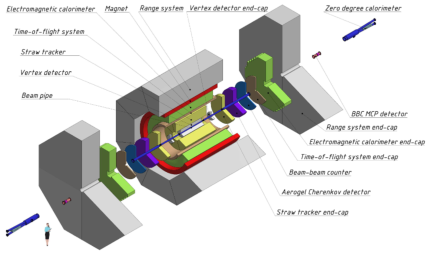
\includegraphics[width=\textwidth]{pictures/detector.pdf}
\caption{\small  General layout of the SPD detector. The picture is taken from Ref.~\cite{TDR_SPD}.} \label{fig:spd_layout}
\end{center}
\end{figure}

 

For the SPD experiment, the NICA collider expects gradual enhancements in its capacity to deliver high energy beams with increasing luminosity. For this reason, the SPD detector operation will be naturally subdivided into different ``stages", with each stage having different collision energies, run conditions, detector setups, and thus essentially different physics programs\cite{TDR_SPD,SPDproto:2021hnm,SPD_1st_stage,Arbuzov:2020cqg}. The starting SPD configuration for the first stage should consist of the solenoidal superconducting magnet, the Range System, the Straw tube-based Tracker, a pair of ZDCs, and a pair of BBCs\cite{TDR_SPD,SPD_1st_stage}. 


For the complete SPD setup, tracking of charged particles and measuring their momenta is going to be performed with a combination of the Silicon Vertex Detector (SVD) and the Straw tube-based Tracking system (ST). However, for the first stage of the SPD operation, the SVD tracker will not be installed, which suggests worsening of the overall momentum resolution, the tracking efficiency, and vertex reconstruction. To provide a performance adequate for the physics tasks, a relatively simple and cheap central tracker based on the Micromegas technology is proposed to be installed as a substitute for the SVD during the first period of data taking. Although the Micromegas-based Central Tracker (MCT) will not be able to provide the accuracy comparable with the SVD tracker, it will allow for improvements in the overall momentum resolution, the tracking efficiency, and vertex reconstruction\cite{TDR_SPD}.


According to Ref.~\cite{TDR_SPD}, partial installation of other detectors (ECal, TOF, etc.) is also possible in the first stage.


It is noteworthy that the SPD detector is optimized for operation at high luminosity but low track multiplicity\cite{TDR_SPD}. For collisions with low multiplicity, event separation can be developed based on interactions between the beam bunches. For $d-d$ collisions at NICA, the time difference between the bunches is expected to be large ($\sim$ 76 ns) with the bunches themselves being sparse. The probability of one interaction per two colliding (overlapping) bunches is about 0.3, which means that not every bunch overlap will deliver an interaction between the beam particles, and if the interaction occurs, it is highly unlikely to have another interaction in the same bunch overlap~\cite{TDR_SPD}. Therefore, detected particles can be attributed to a specific event using the bunch time as reference. Bunch overlaps that did not deliver any interactions can be used to better understand distributions of electronic noise and accidentals, and this information can be further used to deal with background during data analysis. 
%Therefore, interactions of the beam particles are thought to be well-separated in time, and the registered particles can be attributed to a specific event using the bunch time as reference. /check the numbers/




\section{Proton detection}
\label{sec:proton}

The proposed color transparency measurements will require detection of two protons in the reaction final state (denoted $p_{3}$ and $p_{4}$ in Fig.~\ref{fig:diagram}). For the first stage of the SPD operation, proton identification will mostly rely on the information from the Straw system, which will provide track reconstruction (with a spatial resolution about 150 $\mu$m), high precision momentum determination (with the transverse momentum resolution $\sigma_{p_{T}}/p_{T} \approx 2$\% for a particle momentum of 1~GeV/c), and also energy deposition measurements (which will allow for the $\pi$/K/p separation). The information from the Straw system will be supplemented by the MCT signals, which would allow for better proton momentum resolution, tracking, and vertex reconstruction. Also, in case the TOF system is available during the first stage (which is, however, unlikely), it can be used for proton identification, too\cite{TDR_SPD}.


For the proposed measurements, it is important to carefully consider limited particle identification capability of the Straw system. As follows from Fig.~\ref{fig:straw_pid}, the Straw system will be able to adequately perform the $\pi$/K/p separation up to the particle momenta of $\sim$~1.5~GeV/c, while for higher momentum values, reliable separation will be challenging. Therefore, in case the particle identification (PID) relies solely on the Straw system, one should be mindful about requested collision energies of the experiment because for $\sqrt{s_{dd}}\gtrsim$~8~GeV, the corresponding proton momenta will exceed 2~GeV/c, meaning that proper identification of such protons is not probable. The potential (but unlikely) use of the TOF system during the first stage would significantly improve the PID situation as the TOF is expected to provide $\pi$/K/p separation up to a few GeV/c.


It is also noteworthy that (as discussed in Chapter~\ref{chapter_rate}) higher collision energies deliver a larger overall CT contribution and therefore, are generally beneficial for color transparency measurements. At the same time, measurements at smaller collision energies ($\sqrt{s_{dd}}\sim$~8~GeV) are also acceptable as they can still provide a reasonable CT contribution.

\begin{figure}[htp]
\begin{center}
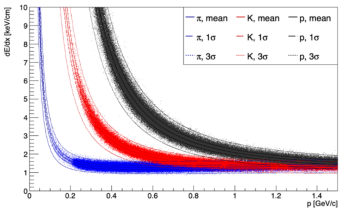
\includegraphics[width=0.6\textwidth]{pictures/straw_pid.pdf}
\caption{\small PID performance in the barrel part of the straw tracker. The dashed and dotted lines indicate 1$\sigma$ and 3$\sigma$ intervals, respectively.  The picture is taken from Ref.~\cite{TDR_SPD}.} \label{fig:straw_pid}
\end{center}
\end{figure}

Another important aspect of the proton identification is that in the $pd\rightarrow ppn$ process, the final protons that managed to avoid interactions with the reaction neutron $p_{s}$ (and thus remained quasi-free) travel in the opposite directions, as was discussed in Ch.~\ref{chapter_generated}. This kinematic feature can be seen as a distinct characteristic trait (kinematic signature) of the quasi-free events of the investigated process and hence can be set as a main selection criterion for the final protons during the data analysis. However, the final protons that participated in soft rescatterings off the neutron $p_{s}$ will deviate from this kinematic pattern due to alterations of their momenta in these interactions. Note that the described kinematic pattern will also be affected by the Fermi smearing. 



\section{Neutron detection}
\label{sec:neutron_det}
    

This section describes the specificities of neutron detection for the proposed color transparency measurements. Depending on the polar angles of the final state neutrons (denoted $p_{s}$ and $p_{s1}$ in Fig.~\ref{fig:diagram}), different detector components can be used for their detection.


According to the Monte Carlo simulation presented in Ch.~\ref{chapter_generated}, the neutron $p_{s}$ generally goes backward/forward with the angle $\widetilde{\theta_{s}}$ varying from 0$^o$ to $\sim$10$^o$. Note that the quantity $\widetilde{\theta_{s}}$ reflects the deviation from the beam axis, and $\widetilde{\theta_{s}} =\left | \theta_{s}^{\textrm{Lab}} \right |$ if the neutron goes forward and $\widetilde{\theta_{s}} = \left | \pi - \theta_{s}^{\textrm{Lab}}\right |$ is the neutron goes backward, while $\theta_{s}^{\textrm{Lab}}$ is the actual neutron polar angle in the Lab system. However, as follows from the weighted histogram in Fig.~\ref{fig:gen_neutrons}, the vast majority of the neutrons will fall in the range 0$^o < \widetilde{\theta_{s}}\lesssim$~3$^o$. It is also important that the neutron polar angle is correlated with its transverse momentum $p_{st}$ as larger values of $\widetilde{\theta_{s}}$ correspond to larger $p_{st}$ values and therefore, to the region with a smaller cross section (see e.g. Fig.~\ref{fig:model}). Therefore, experimental capability of detecting the reaction neutron ($p_{s}$) at different polar angles will reflect how well the $p_{st}$ dependence of the cross section can be measured. 





%The main SPD subdetector to be used to detect reaction neutrons ($p_{s}$) would be the Range system (RS). This subdetector consists of two geometric parts: a cylindrical barrel-shaped part around the beam pipe and the End-Caps, which are vertical disks placed at each open end of the barrel cylinder to capture particles flying out along the beam axis (see Fig.~\ref{fig:spd_layout}). The two RS components will work together to provide full polar angle coverage around the collision point.

%The end caps will be placed at each end of a cylindrical barrel-shaped RS setup to capture particles flying out along the beam axis. 



For larger $\widetilde{\theta_{s}}$ angles (which would correspond to larger $p_{st}$ values and a smaller overall cross section), the reaction neutron ($p_{s}$) is going to be detected in the Range system (RS) of the SPD detector. One can anticipate that neutrons will not give any tracks or signals in the detector components located before the RS but will form showers in the RS. Minimal achievable $p_{st}$ value would then be mainly determined by the geometrical acceptance of the Range system. The projected maximal pseudorapidity for the RS (both barrel and end-cap parts) is currently estimated to be $\eta\simeq 3.14$ (relative to the beam axis), which would correspond to a measurable polar angle range of about 5$^o<\theta_{RS}<$~175$^o$ (in the Lab frame). Note, however, that estimations for the RS minimal/maximal polar angles vary in different studies, e.g. Ref.~\cite{Skachkova:2020zdu} uses the range of 3$^o<\theta_{RS}<$~177$^o$. The measurable angle will also depend on the primary vertex $z$ position at which the interaction occurred as the real beam-crossing region has a gaussian shape along the $z$-axis with $\sigma_{z}\sim$ 30~cm\cite{TDR_SPD,Igamkulov:2019gdu}.


Particle identification in the RS will be performed based on different energy deposition patterns of various particles ($\mu$/p/n). As confirmed by a study performed with the RS testing prototype in 2018, the Range System is expected to provide excellent PID abilities and good quality calorimetry and tracking. For calorimetry, for hadrons with kinetic energies in a range between 1~GeV and 5~GeV, the RS is expected to offer the energy resolution on a level of $\sim$70\% to $\sim$40\%, respectively. The Range System may also provide additional space information – the space angle for a track segment or a shower, and an entry point to the system. See more details in Ref.~\cite{TDR_SPD}.



Meanwhile, for very small angles ($\widetilde{\theta_{s}}\simeq 0^{o}$), which would correspond to small $p_{st}$ values and the region of a very large cross section (see Figs.~\ref{fig:model}~and~\ref{fig:gen_neutrons}), some reaction neutrons ($p_{s}$) can also be detected in the ZDC. %ZDC, however, does not allow for the energy measurements.

  
    
A Zero Degree Calorimeter (ZDC) is a standard device for collider environments. For the SPD experiment, two ZDC devices are supposed to be placed symmetrically about 13 m from the interaction point (on both sides). The strong magnetic field before the ZDC efficiently removes all charged particles, allowing for clean measurements of neutrals. According to Ref.~\cite{TDR_SPD}, the ZDC is expected to have the following performance parameters: time resolution 150-200 ps, energy resolution for neutrons 50-60\%/$\sqrt{E} \bigoplus$ 8-10\%, and neutron entry point spatial resolution 10 mm. Taking that the interaction region of the ZDC is about 10-15 cm, the corresponding maximal detectable polar angle would be about $\widetilde{\theta_{s}}\sim 0.2^{o}-0.3^{o}$.    

From the experimental perspective, kinematic distributions of another neutron involved in the process would be indistinguishable from those of the reaction neutron $p_{s}$. Therefore all detection nuances described above equally apply for both neutrons. However, to extract the $pd\rightarrow ppn$ cross section, one needs to select events in which one of the neutrons remained quasi-free, meaning that it was not involved in any soft rescatterings (in the initial or final state) off other participating nucleons and remained a spectator to the the investigated $p-d$ collision. The neutron that remained quasi-free is denoted as $p_{s1}$ in Fig.~\ref{fig:diagram}. 


Note that for the Monte Carlo simulation presented in Ch.~\ref{chapter_generated}, the $p_{s1}$ neutron was assumed to be quasi-free in the event generator (a spectator to the $pd\rightarrow ppn$ process). For this reason, angular distributions of the $p_{s}$ and $p_{s1}$ neutrons differ in Fig.~\ref{fig:gen_neutrons}.

Meanwhile, when analyzing actual experimental data, selection of events with one quasi-free neutron can be a difficult task. For this purpose, relations presented in Sec.~\ref{sec:topologies} that directly follow from energy-momentum conservation can be of great use as they can help to distinguish between the $p_{s}$ and $p_{s1}$ neutrons and also filter out events in which rescattering of the $p_{s1}$ neutron took place. However, in case the energy-momentum resolution of the experiment is not sufficient for these relations to be employed, selecting the events with one quasi-free neutron may become rather challenging. %See Sec.~\ref{sec:topologies} for details. 



\begin{comment}
    
The detection of another neutron involved in the $pd\rightarrow ppn$ process occurring in $d-d$ collisions (which is denoted as $p_{s1}$ in Fig.~\ref{fig:diagram}) would be beneficial for the proposed color transparency measurements but in general, it is not required (see Section~\ref{sec:topologies} for more details). As follows from the bottom right plot in Fig.~\ref{fig:gen_neutrons}, the neutron $p_{s1}$ goes forward with the polar angles varying in a narrow range 0$^o<\theta_{s1}^{\textrm{Lab}}<$~2$^o$ in the Lab system. The detection of this neutron can also be performed by the ZDC. However, only a small fraction of these neutrons is expected to reach the ZDC due to its very limited geometric acceptance. 

Also note that to produce the plots in Fig.~\ref{fig:gen_neutrons}, the cuts were imposed on the momentum of the deuteron $d_{1}$ in the event generator, to ensure that the neutron $p_{s1}$ goes in the forward direction (see more details in Ch.~\ref{chapter_generated}). Therefore, a small number of neutrons with $\theta_{s1}^\textrm{Lab}>$~2$^o$ are expected to be present in the experiment, and some of them can potentially be detected in the Range system. Events with the $p_{s1}$ neutrons with large polar angles would mostly correspond to the case when rescattering between the neutron $p_{s1}$ and other participating nucleons occurred, and therefore such events will not be of interest for the proposed color transparency measurements. During the data analysis, an additional cut can be performed to eliminated such events, which would allow for a cleaner analyzed event sample. % for the $pd\rightarrow ppn$ process.

Note that for successfully detected neutrons, it is important to distinguish between $p_{s}$ and $p_{s1}$ during the data analysis to ensure correct calculation of the $p_{st}$ variable. In general, this can be done using the relations from Eqs.~\eqref{eq:momenta2} that directly follow from energy-momentum conservation. However, in case the energy-momentum resolution of the experiment is not sufficient for these relations to be employed, the task of distinguishing between $p_{s}$ and $p_{s1}$ may become rather challenging. See Sec.~\ref{sec:topologies} for details.
%provided that the energy-momentum resolution of the experiment is sufficient to 

%For this purpose, the energy-mometumsecond relation in Eqs.~\eqref{eq:momenta2} can be of great use however. See Sec.~\ref{sec:topologies} for details.

\end{comment}

Another possible solution to this issue may be to demand for analysis only those events in which one neutron was detected in the ZDC and the other one -- in the Range system and to claim the former to be the spectator $p_{s1}$ neutron and the latter to be the reaction neutron $p_{s}$. However, taking into account very limited geometric acceptance of the ZDC and the fact that (even quasi-free) neutrons will divert from the precise forward/backward direction due to the Fermi momentum, this method will result in significant suppression in the analyzed statistics and reduced overall analysis flexibility.

It is also noteworthy that larger neutron energies will deliver better energy resolution, meaning that higher collision energies ($\sqrt{s}$) are beneficial for neutron detection. This condition is consistent with the intention to maximize the color transparency contribution (which is larger for larger $\sqrt{s}$ values), but unfortunately, is inconsistent with the optimal conditions for proton identification in the Straw system (which worsens for larger proton energies as described in Sec.~\ref{sec:proton}). Therefore, a reasonable compromise on this matter should be observed.
    
  

  
\begin{comment}
\section{Event separation}

The task of event separation is an important issue that deserves special attention. Unlike electron scattering experiments (where the reference signal for distinguishing one event from another can be derived from the scattered electron as the first-in-time particle), experiments with hadron collisions do not provide such reference for event separation. For this reason, a careful procedure should be developed to attribute registered particles to a specific event.

In general, for hadron colliders, event separation can be achieved by reconstructing the interaction vertex for the registered particles (so that particles that originate from one interaction vertex can be attributed to one event), which is typically performed based on the track fitting procedure (extrapolation). However, this method is well-applicable only for events with large multiplicity (the total number of particles produced in a single collision), which will not be the case for the SPD experiment.  

Meanwhile, for collisions with low multiplicity, event separation may be developed based on interactions between the beam bunches. For $d-d$ collisions at NICA, the time difference between the bunches is expected to be large ($\sim$ 76 ns) with the bunches themselves being sparse. The probability of one interaction per two colliding (overlapping) bunches is about 0.3, which means that not every bunch overlap will deliver an interaction between the beam particles, and if the interaction occurs, it is highly unlikely to have another interaction in the same bunch overlap~\cite{TDR_SPD}.
%Therefore, interactions of the beam particles are thought to be well-separated in time, and the registered particles can be attributed to a specific event using the bunch time as reference. /check the numbers/

Therefore, if electronic noise and accidentals are under control, interactions of the beam particles are thought to be well-separated in time, so that the registered particles can be attributed to a specific event using the bunch time as reference. Additionally, bunch overlaps that did not deliver any interactions can be used to better understand distributions of electronic noise and accidentals, and this information can be further used to deal with the background during the data analysis.

\end{comment}


\section{Reaction topologies}
\label{sec:topologies}

Depending on the number of particles detected in the reaction final state, one can consider working in different reaction ``topologies" during the data analysis. In this section, the following topologies are discussed, the $2p$-topology, the $2p1n$-topology, and the $2p2n$-topology.

The $2p$-topology requires only the detection of the two final state protons ($p_{3}$ and $p_{4}$). The $2p2n$-topology requires the detection of the two protons ($p_{3}$ and $p_{4}$) and the two neutrons ($p_{s}$ and $p_{s1}$) in the final state, while the $2p1n$-topology requires the detection of both protons and the reaction neutron $p_{s}$. See Fig.~\ref{fig:diagram} to recall the particle notations. 



For the $2p$-, the $2p1n$-, and the $2p2n$-topology, respectively, energy-momentum conservation compels the four-momenta of the participating particles to satisfy the following relations.
\begin{equation}
~~~~~~~~~~~~~~~~\left( P_{1}^{\mu}+P_{2}^{\mu}-P_{3}^{\mu} - P_{4}^{\mu} \right)^2~=~0.\\
\label{eq:momenta_new1}
\end{equation}
\begin{equation}
~~~~~~~~~\left( P_{3}^{\mu}+P_{4}^{\mu}+P_{s}^{\mu} -P_{1}^{\mu} -P_{d}^{\mu} \right)^2~=~0.\\
\label{eq:momenta_new2}
\end{equation}
\begin{equation}
\left( P_{3}^{\mu}+P_{4}^{\mu}+P_{s}^{\mu} + P_{s_{1}}^{\mu} - P_{d_{1}}^{\mu}-P_{d}^{\mu}\right)^2~=~0.\\
\label{eq:momenta_new3}
\end{equation}

Here $P_{i}^{\mu}$ are the four-momenta of the particle $i$. For the protons $p_{1}$ and $p_{2}$ in the initial state, note the following, (i) they are assumed to be on-shell and (ii) in the rest frame of the corresponding deuterons, they move with the Fermi momentum.
 

The relations in Eqs.~\eqref{eq:momenta_new1}--\eqref{eq:momenta_new3} allow one to investigate different missing quantities (such as missing masses, energies, or momenta), which can be of great use during the data analysis. If the energy-momentum resolution of the experiment permits, event distributions of the missing quantities can provide additional event selection criteria to separate the events of interest from all other registered events, thus ensuring proper isolation of the $pd\rightarrow ppn$ reaction.

It is noteworthy that Eqs.~\eqref{eq:momenta_new1}--\eqref{eq:momenta_new3} are differently affected by soft rescatterings of the participating nucleons off the neutrons $p_{s}$ and $p_{s1}$. Specifically, soft rescatterings of the protons off both $p_{s}$ and $p_{s1}$ neutrons will introduce distortions into the missing quantities related to Eq.~\eqref{eq:momenta_new1}. However, the missing quantities related to Eq.~\eqref{eq:momenta_new2} will acquire distortions only due to interactions with the neutron $p_{s1}$ but will not be affected by interactions with the neutron $p_{s}$. Finally, interactions with neither the $p_{s}$ nor the $p_{s1}$ neutrons will affect the missing quantities related to Eq.~\eqref{eq:momenta_new3}. See more details in Refs.~\cite{CLAS:2023mfc,my_an_note:2020,my_thesis:2021}.


Furthermore, Eq.~\eqref{eq:momenta_new2} can also allow for distinguishing between the $p_{s}$ and $p_{s1}$ neutrons, which is important for correct calculation of the $p_{st}$ variable. Also note that missing quantities related to Eq.~\eqref{eq:momenta_new1} will benefit from much better resolution than those related to Eq.~\eqref{eq:momenta_new2} and Eq.~\eqref{eq:momenta_new3} because the former relation includes only the proton four-momenta (for the final state), and experimental energy-momentum resolution for protons is expected to be on a decent level. However, due to the fact that the Fermi-momenta of the protons $p_{1}$ and $p_{2}$ (in the initial state) will not be experimentally known, missing quantities related to Eqs.~\eqref{eq:momenta_new1} and~\eqref{eq:momenta_new2} will acquire Fermi smearing. See Refs.~\cite{CLAS:2023mfc,my_an_note:2020,my_thesis:2021,Skorodumina:2015rea, CLAS:2022kta,note_mm_distr} to better understand the specificities of dealing with Fermi-smeared kinematic quantities in data analyses.


It is also important that relations of energy-momentum conservation that sum up to zero (like those in Eqs.~\eqref{eq:momenta_new1},~\eqref{eq:momenta_new2},~and~\eqref{eq:momenta_new3}) are known to deliver the missing quantities that are significantly less sensitive to particle momentum alterations (and therefore form much narrower peaks) than those that peak at non-zero values (like, e.g. in Eqs.~\eqref{eq:momenta2}~and~\eqref{eq:momenta3} from Ch.~\ref{Chap:kin}). More details on that can be found e.g. in Refs.~\cite{CLAS:2023mfc,my_an_note:2020,my_thesis:2021,note_mm_distr}. This peculiar feature can facilitate the use of missing quantities for the event selection even in case of not favorable experimental resolution. Ref.~\cite{note_mm_distr} also describes different factors that typically affect missing mass distributions in experimental studies of exclusive reactions (such as detector resolution, admixtures from other channels, Fermi smearing, and final state interactions with spectator nucleons), which can be of interest for this study, too. Additionally, Ref.~\cite{note_mm_distr} provides some example plots that illustrate the sensitivity of some missing quantities to hadron momentum alterations (which there are assumed to originate from final state interactions but the kinematic study presented in Ref.~\cite{note_mm_distr} is valid for any kind of momentum alterations, including those from the detector resolution).


In general, the data analysis will benefit from using all described reaction topologies in combination. However, it is remarkable that the $2p$-topology alone might already deliver enough information for measurements of the cross section $p_{st}$ dependence. Provided that the final state protons are properly identified, this topology allows one to resconstruct the four-momentum of the reaction neutron $p_{s}$ using energy-momentum conservation as follows,
\begin{equation}
P_{X[s]}^{\mu}= P_{3}^{\mu}+P_{4}^{\mu} -P_{1}^{\mu} -P_{d}^{\mu},\\
\label{eq:mm_neutron}
\end{equation}
where $X$ denotes the undetected part for the reaction $pd\rightarrow ppX$

Note that (as already described above) the reconstructed momentum $P_{X[s]}^{\mu}$ delivered by Eq.~\eqref{eq:mm_neutron} will be Fermi-smeared and affected by soft rescatterings of the protons off the neutron $p_{s1}$, but its overall resolution is expected to be on a reasonable level. In addition to that, since this method does not require neutron detection, it can be used to perform measurements in the $p_{st}$ ranges that are inaccessible in topologies with a neutron detection (due to limitations in geometric acceptance of the RS and the ZDCs).  




